\chapter{Design}

\section{The Language}
The idea was to think of a language that could implement all the possible actions which a security tester would be wanting to do on a multipart webapp test.\\
I had to decide how to write and define the actual tests, i thought i could define a proper language with a dedicated parser, but it was not worth the effort, as there are already some well-tested alternatives available. I found a great alternative: i used JSON as a base over which write the tests. It is a convinient way of defining gerarchical sturctures like tests could be.
The gerarchical structure and the details of the language will be discussed in the next charapter.

\subsection{Language structure}
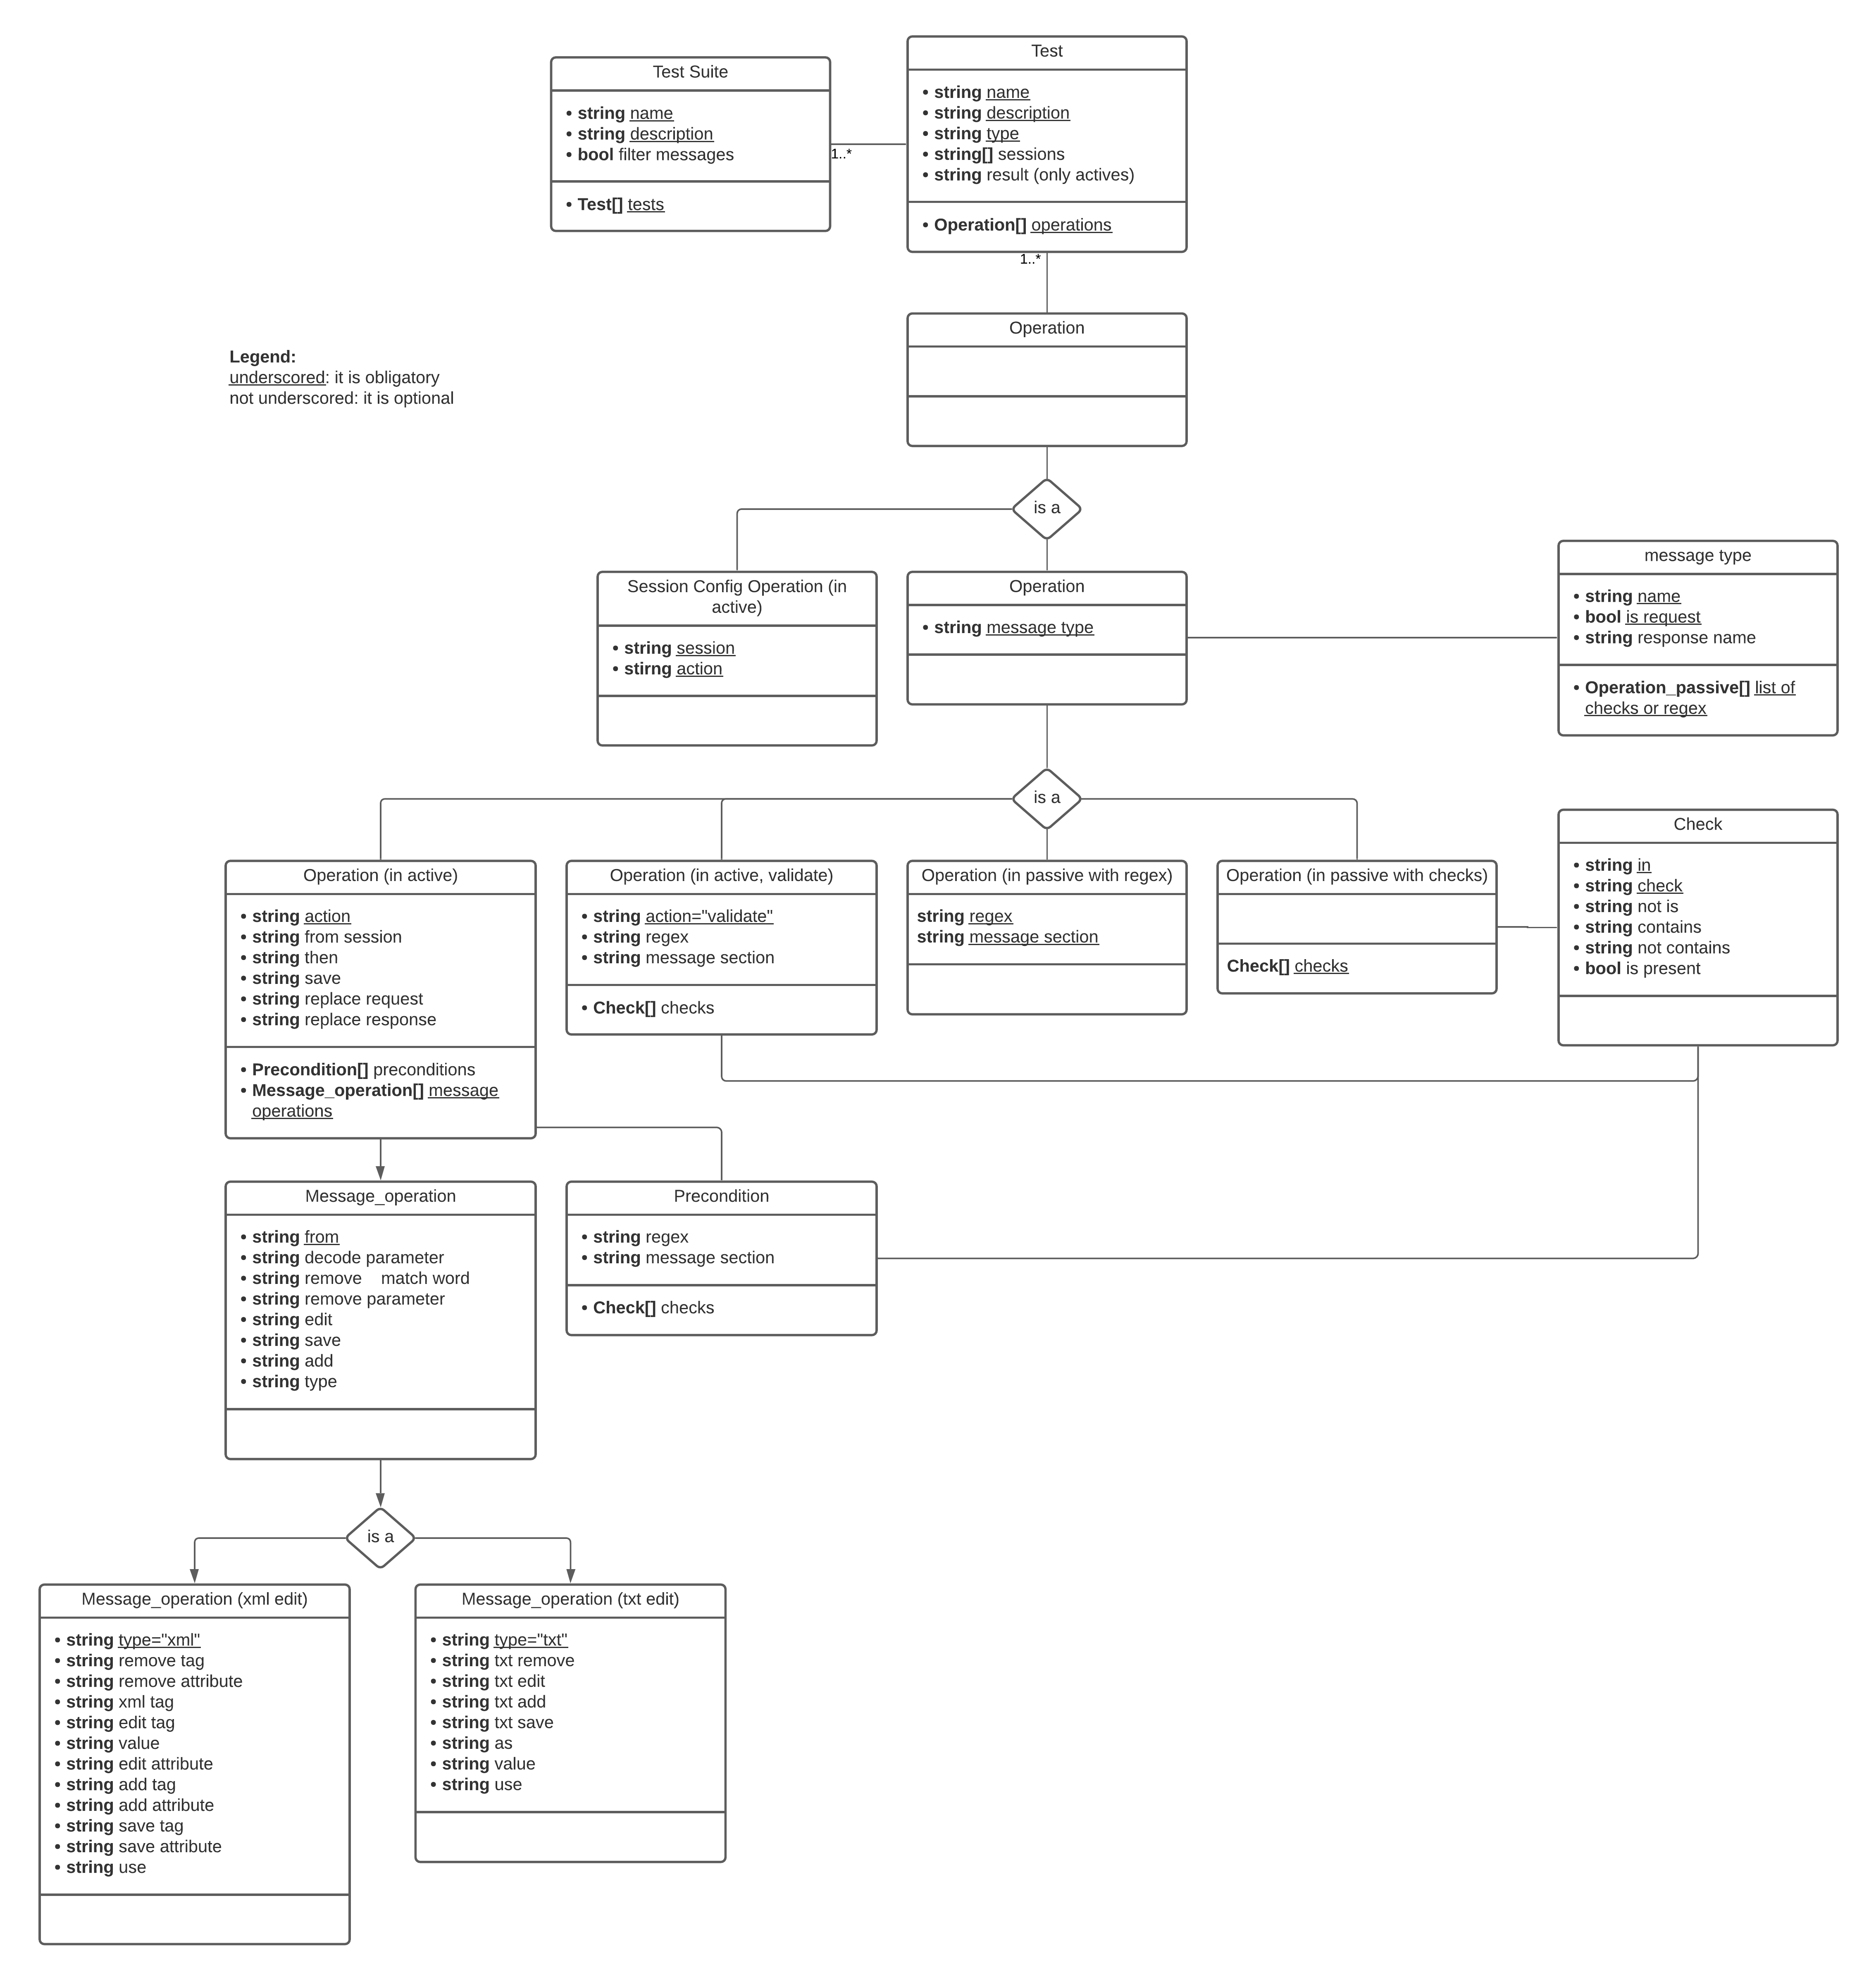
\includegraphics[width=\textwidth]{language_structure.png}

\subsubsection{Test suite}
The test suite is the main component which contains all the other one, it is composed by:
\begin{itemize}
    \item Test suite name, the name of the test suite
    \item Test suite description, the description of the test suite
    \item Tests, which is a list containing the tests to be executed
\end{itemize}

\subsubsection{Test}
The Test object is the one that actually defines a test. As said earlier, a test is contained in a Test Suite, and has various items:
\begin{itemize}
    \item name
    \item description
    \item type, it can be "active" or "passive"
    \item sessions, which is a list of the sessions which are needed in this test
    \item result, (only for actives) it defines the conditions over which the test is considered passed or not.
    \item operations, a list of operation objects which will be executed in the Test object
\end{itemize}

it can be defined either as an active or a passive test, depending on the type of actions it has to do on the intercepted messages. If a doesn't need to manipulate the flow or the content of the messages, then it is considered passive, otherwise it is considered active.
The list of operations is executed iteratively one after the other.

\subsubsection{Operation}
The operation object is the thing that define what a test actually does. As shown in the image above, an operation could be either a standard operation or a session config operation, the latter is used to manage the sessions for the active tests (i.e. start, stop, pause). Depending on the type of test which an Operation is defined into, the standard Operation can be active or passive.
\\A \textbf{passive} operation should contain one of the following options:
\begin{itemize}
    \item A list of Check objects
    \item A regex inspection
\end{itemize}
A regex operaton executes an inspection in


\section{The oracle}


